\documentclass{article}

\usepackage[utf8]{inputenc}
\usepackage[spanish]{babel}

\usepackage{caratula}

\usepackage{subcaption}
\usepackage{graphicx}
\usepackage{subfig}
\usepackage{dirtytalk}
\usepackage{enumerate}

\usepackage{amssymb}
\usepackage{mathtools}
\usepackage{amsmath}
\usepackage{amsthm}

\usepackage{algorithm}
\usepackage{algpseudocode}
\usepackage{listingsutf8}

\usepackage{float}
\floatplacement{figure}{h!}

\usepackage{geometry}
\usepackage{fixltx2e}
\usepackage{wrapfig}
\usepackage{cite}
\usepackage{dsfont}
\usepackage{ulem}

\usepackage[space]{grffile}

\geometry{
 a4paper,
 total={210mm,297mm},
 left=30mm,
 right=30mm,
 top=30mm,
 bottom=30mm,
 }
 
\usepackage{booktabs}
 
% sql stuff
\usepackage{listings}
\usepackage{courier}
\usepackage{pdflscape}

\lstdefinestyle{SQL}
{%
  language   = SQL,
  basicstyle = \small\ttfamily,
  columns    = fixed,
}

\lstset{style=SQL}
 
\newtheorem{theorem}{Teorema}[section]
\newtheorem{corollary}{Corolario}[theorem]
\newtheorem{lemma}{Lema}[theorem]
 
\theoremstyle{definition}
\newtheorem{definition}{Definición}[section]
 
\theoremstyle{remark}
\newtheorem*{remark}{Observación}

\usepackage[dvipsnames]{xcolor}
 
\begin{document}
% Estos comandos deben ir antes del \maketitle
\materia{Bases de Datos} % obligatorio

\titulo{RTP 1 \\ Grupo 11}
\subtitulo{Sistema de Seguimiento de Casos Policiales \\ \today}
\grupo{}

\integrante{Julián Bayardo}{850/13}{julian@bayardo.com.ar} % obligatorio
\integrante{Christian Cuneo}{755/13}{chriscuneo93@gmail.com} % obligatorio 
\integrante{Mauro Cherubini}{835/13}{cheru.mf@gmail.com}
\integrante{Martin Baigorria}{575/14}{martinbaigorria@gmail.com}
 
\maketitle

\tableofcontents

\pagebreak

\section{Introducción}

En una provincia de la República Argentina se desea actualizar el sistema informático para llevar un mejor registro de los casos criminales que se producen y su respectiva información asociada. Para ello, se nos ha solicitado modelar la estructura del problema utilizando un Modelo Entidad Relación (MER). Para ello utilizaremos la técnica de Diagramas de Entidad Relación (DER). Una vez que finalizada esta estructura, pasaremos de este diseño conceptual al diseño lógico utilizando el Modelo Relacional (MR), identificando cuidadosamente las claves primarias y foráneas que utilizaremos. Luego implementaremos este diseño utilizando el motor de bases de datos PostgreSQL, elegido por su facilidad para ser desplegado y su amplia cantidad de documentación y conocimiento público al respecto.

\subsection{Requerimientos}

A continuación listamos los requerimientos del sistema, según logramos extraer de la consigna:

\begin{itemize}
    \item De cada caso se precisa registrar:
        \begin{enumerate}
            \item Fecha y hora del suceso.
            \item Fecha de ingreso.
            \item Descripción del caso.
            \item Lugar del suceso.
            \item Categoria (secuestro, homicidio, robo, etc).
            \item Personas involucradas.
            \item Oficiales involucrados.
            \item Estado del caso (resueltos, pendientes, congelados o descartados).
        \end{enumerate}
        En cuanto a los oficiales involucrados, uno debe ser investigador principal mientras que el resto trabaja como auxiliar.
    \item Dependiendo del estado del caso, se deben guardar diferentes datos. Los casos resueltos deben contar con:
        \begin{enumerate}
            \item Descripción de la resolución.
            \item Personas culpables.
        \end{enumerate}
    Los casos congelados deben contar con:
        \begin{enumerate}
            \item Fecha en que se congelo.
            \item Comentario.
        \end{enumerate}
    Para los casos descartados se debe registrar:
        \begin{enumerate}
            \item Motivo.
            \item Fecha de descarte.
        \end{enumerate}
    Finalmente para los casos resueltos se debe contar con:
        \begin{enumerate}
            \item Fecha de resolución.
            \item Oficial que cerro el caso.
        \end{enumerate}
    \pagebreak
    \item De las personas se precisa saber:
        \begin{enumerate}
            \item DNI.
            \item Nombre.
            \item Apellido.
            \item Domicilio.
            \item Fecha de nacimiento.
            \item Teléfonos. Los teléfonos pertenecen a las siguientes categorías.
                    \begin{itemize}
                        \item Celular.
                        \item Fijo.
                        \item Laboral.
                        \item Domiciliario.
                        \item Otras.
                    \end{itemize}
            \item Casos en los que esta o estuvo involucrado.
        \end{enumerate}
    Tener en cuenta que en un domicilio pueden convivir diferentes personas.
    \item En un caso, las personas pueden cumplir con uno de los siguientes roles:
        \begin{enumerate}
            \item Víctima.
            \item Testigo.
            \item Otros.
        \end{enumerate}
    \item Algunas de las personas involucradas en un caso son oficiales de policía, de los cuales se necesitan saber los siguientes datos:
        \begin{enumerate}
            \item Número de placa.
            \item Fecha de ingreso.
            \item Numero de escritorio asignado.
            \item Servicio prestado.
            \item Departamento al que pertenece.
            \item Rango (teniente, sargento, etc)
            \item Testimonios tomados.
        \end{enumerate}
    Un oficial posee un rango especifico, pero puede haber muchos oficiales con el mismo rango.
    \item De cada departamento policial se necesita saber:
        \begin{enumerate}
            \item Nombre.
            \item Dirección.
            \item Localidad.
            \item Una o mas lineas telefónicas para comunicarse.
            \item Departamentos a los que supervisa.
        \end{enumerate}
    \item Para un caso las personas involucradas pueden tener un conjunto de eventos que formaría una linea de tiempo que se relaciona con el caso. Para cada evento se desean registrar:
        \begin{enumerate}
            \item Fecha y hora del evento.
            \item Descripción.
        \end{enumerate}
    \pagebreak
    \item Algunas personas pueden presentar un testimonio o declaración para un caso en particular. De este testimonio se debe registrar:
        \begin{enumerate}
            \item Fecha y hora  del testimonio.
            \item Texto del testimonio.
            \item Oficial encargado.
        \end{enumerate}
    \item Cada caso puede tener evidencia. De la evidencia se deben recolectar:
        \begin{enumerate}
            \item Fecha y hora en que se la encontró.
            \item Descripción.
            \item Cadena de custodia (lugares por los que paso).
        \end{enumerate}
    \item Por otro lado, para cada movimiento de lugar en la cadena de custodia se deben registrar:
        \begin{enumerate}
            \item Fecha y hora del movimiento.
            \item Oficial a cargo.
            \item Comentario.
            \item Lugar por el que paso.
        \end{enumerate}
\end{itemize}

\subsection{Suposiciones y Conocimiento de Dominio}


Suposiciones y Conocimiento de Dominio:
Durante la modelización del DER nos encontramos con toda un serie de obstáculos para los cuales tuvimos que realizar toda una serie de consideraciones:

\begin{itemize}
\item Dado que un caso podría encontrarse en 4 diferentes instancias disjuntas (Pendiente, Descartado, Congelado, o Resuelto), y a su vez cada uno de ellas demandaba algún tipo de apreciación diferente no solo, en un sentido semántico sino también implémentatelo. Esto último se hizo evidente en en algunos datos de interés, como la fecha de resolución de un caso, que es inherente a un caso resuelto, pero carece de sentido para un caso pendiente. A su vez muchos otros datos caracterizan a un caso de manera mas general, siendo por ejemplo una descripción, fecha de ingreso, y de suceso, algunos de ellos. Teniendo todo esto en cuenta nos pareció lo mas conveniente realizar una jerarquía disjunta, con una superentidad Caso y otras 4 subentidades que representen las instancias del mismo.

\item Dado que se necesitaba registrar toda la gente involucrada en un caso, diseñamos una entidad Persona que se relaciona con el Caso; y debido a que era de vital interés destacar entre las personas involucradas, a aquellas que ofician de policía, decidimos realizar una entidad Oficial que tuviera como superentidad a Persona en una jerarquía de cobertura opcional. De esta forma todo oficial seria registrado como persona, pero obviamente no toda persona sería policía.

\item Consideramos que para cada caso en particular, una persona podría tener un solo rol. Por ello decimos diseñar una relación ternaria entre Caso, Persona y Rol, de manera que para cada par Caso-Persona, hubiera un único rol.

\item En caso de los oficiales se nos pedía almacenar cuales estaban investigando cada caso, y de entre todos ellos cual era el principal. Para ello consideramos a tener un rol llamado Investigador, que caracteriza a todos los oficiales que investigan en dicho caso. Para el caso del oficial principal destacamos su importancia del resto de los investigadores en sus respectivos casos mediante una relación directa entre Caso y Oficial.

\item Interpretamos que para cada par caso-persona, podrían llegar a haber varios testimonios y varios eventos (pudiendo no haber ninguno). Debido a la opcional pero dependiente relación decidimos representar ambas por medio de dos entidades diferente que se asocian a al par caso-persona por medio de una agregación para cada una. Debido a que por decisión de la cátedra una relación ternaria no puede verse involucrada con una agregación, decidimos crear una nueva relación llamada \textit{participa}; la idea detrás de ella es relacionar por medio de ella a los casos con sus respectivas personas que hayan participado en algún evento o presentado un testimonio (para su correspondiente caso). Los testimonios además debían ser tomados por un oficial, al cual por ende relacionamos por medio de una relación Oficial-Testimonio.

\item Para el caso de los teléfonos y ubicación también diseñamos entidades acordes, si bien en principio estos podrían parecer atributos decidimos modelarlos como entidades para eliminar redundancia de datos; recordemos que mas de una persona podía vivir en un mismo lugar (habría mucha repetición del mismo valor en el hipotético atributo de la tabla Persona), y por el lado del teléfono: una persona podía tener vario teléfonos (y de distinto tipo), resultaba medio complicado expresarlo con un atributo multivaluado, además el las tablas resultantes no nos dejarían algo del todo normalizado. Debido a además no necesitábamos que cada persona y departamento tuviera al menos un teléfono, pero que un mismo teléfono no perteneciera tanto a una persona como a un departamento (pero si a uno de los dos), diseñamos una jerarquía con teléfono, diferenciando así los teléfonos personales de los teléfonos departamentales, pero manteniendo la características comunes de todo teléfono. Análogamente para las ubicaciones, en vez de usar atributos para almacenar la calle, numeración, localidad, etc, decidimos generar tablas para cada uno de ellos.
\end{itemize}

\pagebreak

\section{Modelo de Entidad Relación}

\subsection{Diagrama de Entidad Relación}

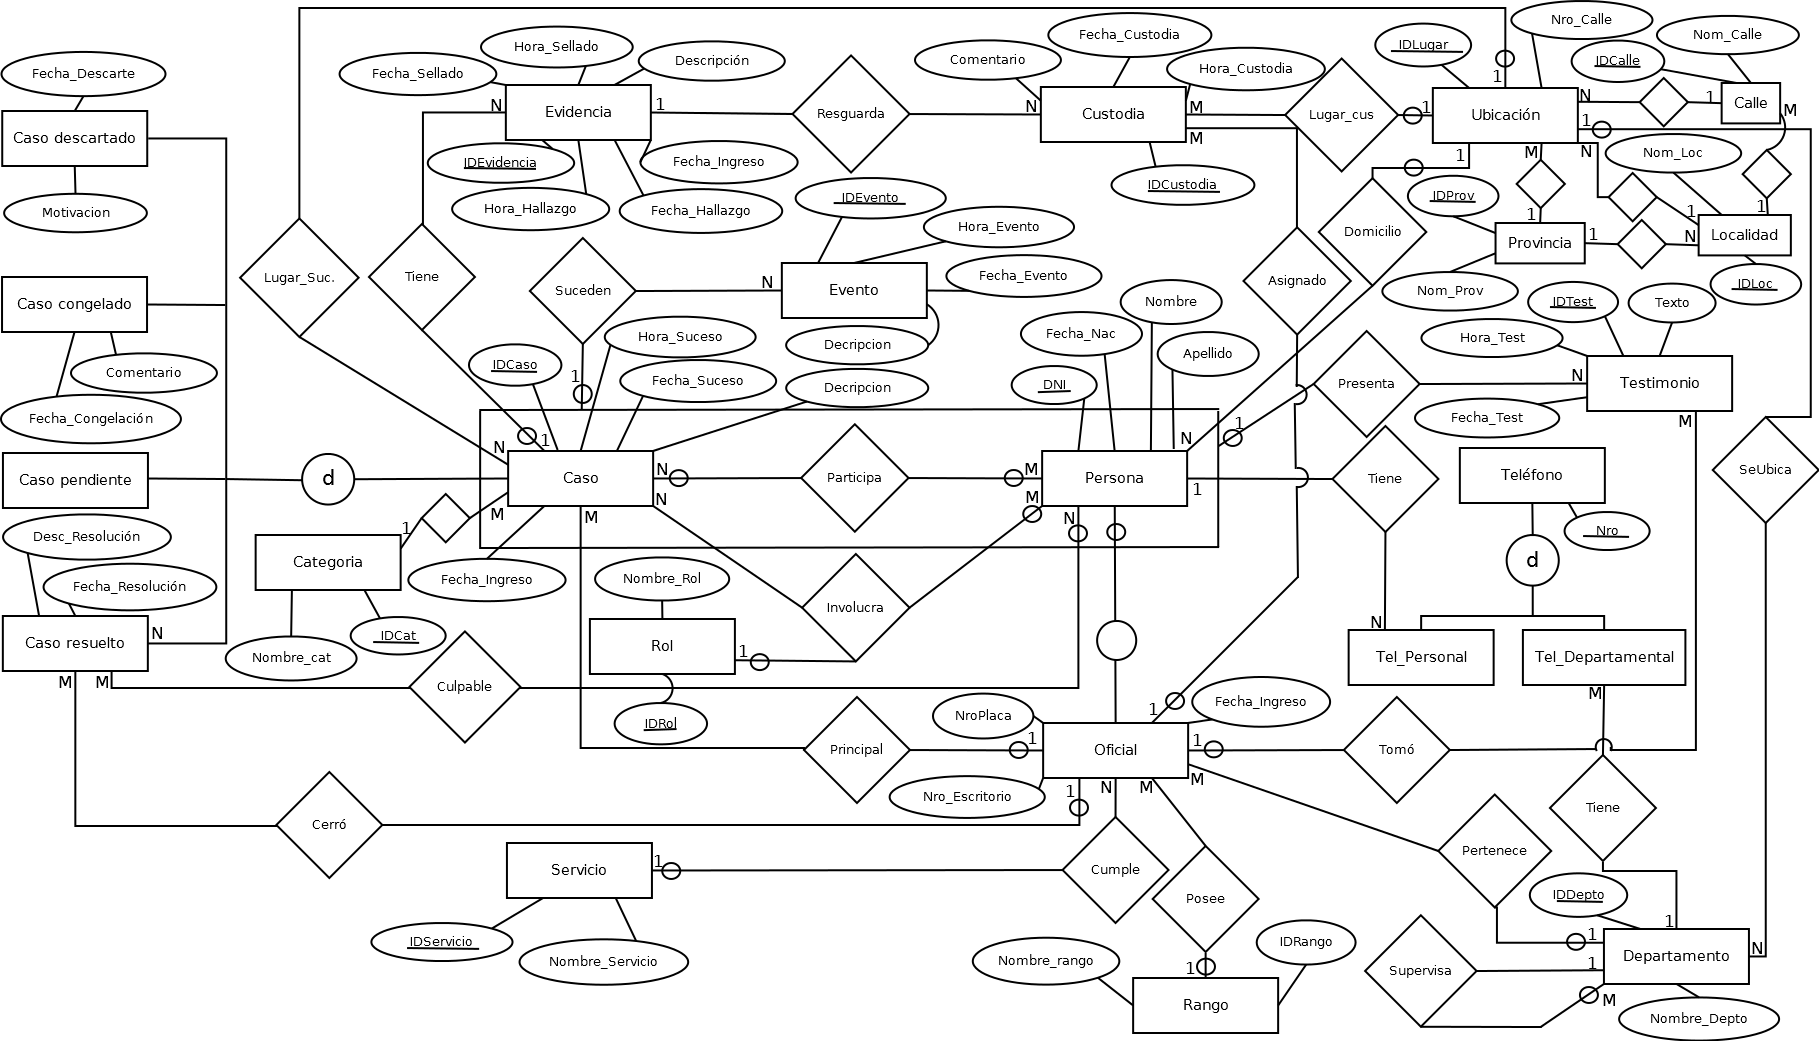
\includegraphics[width=\textheight,height=\textwidth*11/10,angle=90]{der.png}

\section{Modelo Relacional}

Una propiedad interesante de los Diagramas de Entidad Relación es que, una vez diseñados, pasar al Modelo Relacional es simplemente un paso mecánico. Luego, en caso de no poder hacer algún tipo de consulta, eso nos indica que el diseño inicial probablemente estaba incompleto, lo que nos lleva a un mejor entendimiento del problema. A continuación mostramos el Modelo Relacional, con sus respectivas claves primarias y foraneas.

\begin{enumerate}
\item \textbf{Calle} (\underline{idcalle}, nomcalle, \dotuline{idloc})
\item \textbf{Caso} (\underline{idcaso}, descripcion, fecha\_ingreso, fecha\_suceso, hora\_suceso, tipo, \dotuline{oficialprincipaldni}, \dotuline{id\_ubicacion}, \dotuline{id\_categoria})
\item \textbf{CasoCongelado} (\dotuline{\underline{idcaso}}, comentario, fecha\_congelacion)
\item \textbf{CasoDescartado} (\dotuline{\underline{idcaso}}, fecha\_descarte, motivacion)
\item \textbf{CasoResuelto} (\dotuline{\underline{idcaso}}, desc\_resolucion, fecha\_resolucion, \dotuline{oficialresueltodni})
\item \textbf{Categoria} (\underline{idcat}, nombre\_cat)
\item \textbf{Culpable} (\underline{\dotuline{idcaso}, \dotuline{personadni}})
\item \textbf{Custodia} (\underline{idcustodia}, \dotuline{idevidencia}, \dotuline{oficialdni}, \dotuline{id\_ubicacion}, comentario, fecha\_custodia, hora\_custodia)
\item \textbf{Departamento} (\underline{iddepto}, nombre\_depto, \dotuline{supervisor}, \dotuline{id\_ubicacion})
\item \textbf{Evento} (\underline{idevento}, \dotuline{idcaso, personadni}, descripcion, hora\_evento, fecha\_evento)
\item \textbf{Evidencia} (\underline{idevidencia}, \dotuline{idcaso}, fecha\_sellado, hora\_sellado, descripcion, fecha\_ingreso, fecha\_hallazgo, hora\_hallazgo)
\item \textbf{Involucra} (\underline{\dotuline{idcaso}, \dotuline{personadni}}, \dotuline{idrol})
\item \textbf{Localidad} (\underline{idloc}, nom\_loc, \dotuline{idprov})
\item \textbf{Oficial} (\dotuline{\underline{dni}}, \dotuline{idservicio}, \dotuline{iddepto}, \dotuline{idrango}, fecha\_ingreso, nroplaca, nro\_escritorio)
\item \textbf{Participa} (\underline{\dotuline{idcaso}, \dotuline{personadni}})
\item \textbf{Persona} (\underline{dni}, fecha\_nac, nombre, apellido, tipo, \dotuline{id\_ubicacion})
\item \textbf{Provincia} (\underline{idprov}, nom\_prov)
\item \textbf{Rango} (\underline{idrango}, nombre\_rango)
\item \textbf{Rol} (\underline{idrol}, nombre\_rol)
\item \textbf{Servicio} (\underline{idservicio}, nombre\_servicio)
\item \textbf{Telefono} (\underline{nro}, tipo)
\item \textbf{TelefonoDepartamental} (\dotuline{\underline{nro}}, \dotuline{iddepto})
\item \textbf{TelefonoPersonal} (\dotuline{\underline{nro}}, \dotuline{personadni})
\item \textbf{Testimonio} (\underline{idtest}, \dotuline{personadni,idcaso}, \dotuline{oficialdni}, texto, hora\_test, fecha\_test)
\item \textbf{Ubicacion} (\underline{id\_lugar}, \dotuline{idcalle}, nro\_calle, \dotuline{idloc}, \dotuline{idprov})
\end{enumerate}
\pagebreak

\subsection{Restricciones}

Las siguientes restricciones aplican sobre el Modelo Racional (además de las determinadas en el DER). Las enunciamos sobre las tablas directamente por considerarlo más fácil para comprender las motivaciones.

En todos los items que siguen, cuando decimos que un "nombre es normalizado" nos referimos a que utilizamos una única convención; por ejemplo, la primer letra es mayúscula y el resto minúsculas para todo el string. Esto nos permite asegurar que el UNIQUE constraint del motor de la base de datos sea efectivo.

\begin{enumerate}
    \item Los nombres de cada calle son únicos y normalizados.
    \item Todo oficial que figura como oficial principal de un caso también figura relacionado con el por la relación Involucra. Además el rol de ese oficial en particular debe ser el de Investigador para dicho caso.
    \item Ninguna persona que no sea oficial puede tener como rol Investigador.
    \item Cada oficial que toma algún testimonio en cierto caso, debe figurar como investigador del mismo caso por medio del rol Ivestigador.
    \item Ningun oficial puede tomarse testimonio a si mismo; si un oficial presenta testimonio se lo debe tomar otro oficial.
    \item Todo caso fue ingresado después del momento del suceso.
    \item El tipo de un caso es menor o igual a 3. Además, el oficial principal asignado al caso ingresó a la fuerza luego de que el caso haya sido ingresado en el sistema.
    \item El tipo de un caso pendiente es 0.
    \item Toda persona que se relaciona con un caso por medio de la relación \textit{participa}, debe haber presentado un testimonio para dicho caso, o en su defecto tener asociado algún evento para dicho caso.
    \item Toda persona que se relaciona con un caso por medio de la relación \textit{participa} debe relacionarse con dicho caso también por medio de la relación \textit{involucra}.
    \item La fecha de congelación de un caso congelado es mayor o igual a la fecha en la que sucedió el caso. Además, el tipo de un caso congelado es 1.
    \item La fecha de descarte de un caso descartado es mayor o igual a la fecha en la que sucedió el caso. Además, el tipo de un caso descartado es 2.
    \item La fecha de resolución de un caso resuelto es mayor o igual a la fecha en la que sucedió el caso. Además, el tipo de un caso resuelto es 2. Fuera de eso, el oficial que resolvió el caso debe tener una fecha de ingreso mayor o igual a la fecha en la que sucedió el caso.
    \item Los nombres de cada categoría son únicos y normalizados.
    \item El oficial que realiza una custodia ingreso a la fuerza antes del comienzo de la custodia. Además, la evidencia que es custodiada fue hallada antes que el comienzo de la custodia.
    \item Una evidencia puede ser parte de una única custodia para cualquier momento en el tiempo. Además, una evidencia no puede estar en más de una ubicación en ningún momento dado.
    \item Un oficial no puede ser parte de dos custodias que sucedan en ubicaciones separadas en ningún momento.
    \item El nombre de un departamento está siempre normalizado. Además, es único para cada ubicación.
    \item Todo evento debe suceder luego de que el caso al que refiere haya sido ingresado.
    \item Para un mismo par caso y persona, no puede haber mas de un evento con la misma fecha y horario.
    \item El hallazgo de una evidencia debe suceder luego de que el caso haya sido creado, y su sellado luego de su hallazgo.
    \item El nombre de una localidad es único por provincia, y además está normalizado.
    \item El tipo de una persona que no es oficial es 0.
    \item El número de placa y escritorio de un oficial son únicos. Además, el tipo de un oficial es 1.
    \item El nombre de una provincia es único y está normalizado.
    \item El nombre de un rango es único y está normalizado.
    \item El nombre de un rol es único y está normalizado.
    \item El nombre de un servicio es único y está normalizado.
    \item El tipo de un teléfono es o bien 0, o bien 1. Además, cada número es único.
    \item El tipo de un teléfono departamental es 1.
    \item El tipo de un teléfono personal es 0.
    \item El horario de un testimonio es mayor al ingreso del oficial que lo tomó, y mayor al momento en que sucedió el caso.
    \item Un oficial no puede tomar más de un testimonio en un determinado momento.
    \item Una persona no puede dar más de un testimonio en un determinado momento.
    \item La 3-upla determinada por una calle, su altura, y la localidad determinan unívocamente a una ubicación, de la misma forma en que lo hace su id.
\end{enumerate}

Lamentablemente, el haber decidido utilizar MySQL fue una mala estrategia pues no tenemos forma de utilizar CHECK CONSTAINTs en ella, es decir, no podemos forzar al motor a verificar las restricciones más simples de una forma conveniente. La única forma de verificar las mismas es utilizando Triggers, y por cada condición verificada tener dos: uno para antes del INSERT, y uno para antes del UPDATE; resultando en una duplicación de código realmente muy poco elegante y práctica.

\pagebreak

\section{Implementación Física y Funcionalidades}

Los archivos SQL para recrear la base de datos están disponibles junto con los archivos entregados. El archivo más conveniente (pues levanta toda la base de datos sin ningún problema) es full\_database\_dump.sql; este archivo, creado con pg\_dump, debería funcionar sin ningún inconveniente. Por otro lado, en caso de tener un cliente que no soporte la sintaxis utilizada por pg\_dump, el archivo schemas.sql levanta las tablas y sus restricciones, mientras que los archivos en individual\_data\_dump levantan los datos.

Sugerimos fuertemente utilizar la herramienta DataGrip como cliente, pues los datos fueron generados y testeados utilizando la misma; y podemos asegurar que funciona correctamente.

\subsection{Funcionalidades}

\begin{enumerate}
    \item Datos de las personas que fueron sospechosas.
    \item Direcciones donde convivieron personas sospechosas de diferentes casos.
    \item Oficiales que participaron en la cadena de custodia de evidencias para más de un caso.
    \item La sucesión de eventos de personas involucradas en un caso.
    \item Un ranking de oficiales exitosos, es decir los que cerraron mayor cantidad de casos (resueltos).
    \item Las ubicaciones de todas las evidencias de un caso.
    \item La lista de oficiales involucrados en un caso.
    \item Las categorías de casos ordenadas por cantidad de casos.
    \item Todos los testimonios de un caso dado.
    \item Para una categoría en particular listar, para cada uno de los casos, los testimonios asociados.
\end{enumerate}

\lstinputlisting[style=sql]{queries.sql}

\pagebreak

\section{Conclusiones}

En la practica, muchas veces se pasa directamente desde una idea vaga del un problema al esquema de la base de datos. Luego este esquema se modifica de manera incremental hasta que cumple con los requerimientos del problema. En este trabajo practica exploramos el Modelo de Entidad Relación. Este modelo nos permite formalizar nuestra idea del problema por medio de entidades y relaciones entre las mismas. De esta manera, antes de comenzar la implementación uno tiene una idea global de como están distribuidos los datos, lo que lleva no solo a una mejor comprensión del problema si no que también a un diseño mas eficiente y robusto ante futuros cambios. La ventaja adicional es que al tener un esquema del funcionamiento de toda nuestra base de datos, otros desarrolladores que en un futuro quieran hacer una modificación rápidamente pueden obtener una visión global de como están organizados los datos.

Una propiedad interesante de los Diagramas de Entidad Relación es que, una vez diseñados, pasar al Modelo Relacional es simplemente un paso mecánico. Luego, en caso de no poder hacer algún tipo de consulta, eso nos indica que el diseño inicial probablemente estaba incompleto, lo que nos lleva a un mejor entendimiento del problema.

En este trabajo exploramos ambas técnicas exitosamente: planteamos un diagrama de entidad relación, hicimos su correspondiente modelo relacional, planteamos las restricciones adicionales inherentes problema, así como las restricciones inherentes al modelo relacional para corresponderse con la situación modelada, tomamos la encarnación del modelo en un sistema de base de datos, lo llenamos con datos de test, y generamos consultas sobre el mismo como verificaciones de correctitud del modelo.

Si bien no realizamos un trabajo de normalización de la base de datos -que a priori es necesario porque la traducción del DER en un MR no garantiza una organización óptima de los datos en el sentido de las formas normales-, intentamos en todos los casos minimizar las claves primarias, respetar las dependencias funcionales, y minimizar la redundancia de datos.

\end{document}